\documentclass[../notes.tex]{subfiles}
\graphicspath{{\subfix{../img/}}}
\begin{document}

\section{Background}
Some background information must be understood before delving into control theory.
\subsection{Calculus}
I am not trying to rewrite a textbook here, nor do I have to knowledge to. This will just be a quick refresher on the most important topics.
\subsubsection{Differentiation}
\subsubsection{Integration}

\subsection{Differential Equations}
\subsubsection{Ordinary (ODE)}
\subsubsection{Partial (PDE)}
\subsubsection{Jacobian Matrix} \label{sec:jacobian}

\subsubsection{Convolution}
Convolution integrals are useful for solving initial value problems with general forcing functions.
\begin{equation}
    (f * g)(t) = \int_{0}^{t} f(t-\tau)g(\tau)d\tau
\end{equation}

\subsubsection{Fourier Transforms}
Any periodic function can be represented by a Fourier series (series of periodic functions).

For periodic functions that decay to zero, we can use the Fourier transform.
\begin{equation}
    f(w) = \int_{-\infty}^{\infty}f(t)e^{-iwt}dt
\end{equation}
This transform converts a continuous time domain signal into a continuous frequency domain signal. In other words, it converts a signal into its component frequencies.

\subsubsection{Laplace Transforms}
The Laplace transform is a more general case of the Fourier transform.

\paragraph{Transfer Functions}
Applying the Laplace transform to a time domain function will produce the frequency domain representation of that function, also known as a transfer function.

\paragraph{Geometry of Transfer Functions}

\subsubsection{Delayed Differential Equations}

\subsubsection{Poles \& Zeros}
The poles and zeros of a transfer function provide some critical information

\subsection{Linear Algebra}
\subsubsection{Basic Operations}
\subsubsection{Matrix Inversion}
\subsubsection{Eigenvectors \& Eigenvalues} \label{sec:eig}


\subsection{Mechanics (Newtonian)}
Understanding the physics that inform the behavior of a system is critical to modeling and controlling it.
\begin{description}
    \item[Newton's 1st Law]
    \item[Newton's 2nd Law]
    \item[Newton's 3rd Law]  
\end{description}
\subsubsection{Linear}
\subsubsection{Rotational}
\paragraph{Coriolis Force}
The presense of rotation adds an additional (faux) force. This is described further in (\underline{\ref{sec:coriolis}}).
\subsubsection{Electrical}
Electrical circuits can be modeled very similarly to the mechanical system. The classic example is RLC (resistor-inductor-capacitor) circuits.


\subsection{Lagrangian Mechanics}
Lagrangian mechanics are preferable to use for dynamical systems that have multiple components whose interaction is complicated to express (eg. multi-body systems). This is especially true if internal reactions are not of immediate interest.
\begin{equation} \label{eq:lagrangian}
    \text{Action: } S = \int_{t_1}^{t_2} L(q, \dot{q})dt
\end{equation}
Where $L(q, \dot{q})$ is the Lagrangian and $q\in \mathbb{R}^{nq}$ is a vector of generalized degrees of freedom (positions, angles). $\dot{q}$ is the vector of corresponding rates of change of the degrees of freedom (linear + angular velocities).
\begin{equation}
    L(q, \dot{q}) = T(q, \dot{q}) - V(q)
\end{equation}
$T(q, \dot{q})$ is the kinetic energy function, $V(q)$ is the potential energy function. Thus the Lagrangian is the difference between the system's total kinetic and total potential energy.
\paragraph{Principle of Least Action} A conservative system (one that does not gain or lose energy) starting in state $q(t_1)$ at time $t_1$ and ending at state $q(t_2)$ at time $t_2$ follows a path that makes the action $S$ stationary (first derivative goes to zero). This is the path of least action. While the path of least action minimizes the action the vast majority of the time, the stationary condition does not guarantee minimization.
\paragraph{Euler-Lagrange Equations for Conservative Systems} The path of least action can be thought of as a continuous steam of states $q(t)$ over the time interval. It must satisfy the Euler-Lagrange Equations.
\begin{equation} \label{eq:eulerLagrangeCons}
    \frac{d}{dt}(\frac{\partial L}{\partial \dot{q}_j}) - \frac{\partial L}{\partial q_j} = 0, \quad j \in \{1, ..., n_q\}
\end{equation}
This yields $n_q$ equations of motion, one corresponding to each of the generalized degrees of freedom. This we obtain all the equations of motion necessary to describe a conservative (energy-preserving) dynamical system.
\paragraph{Euler-Lagrange Equations for Non-conservative Systems} We can modify Eq. \ref{eq:eulerLagrangeCons} to account for energy dissipation (eg. friction) and energy (eg. forcing).
\begin{equation}
    \frac{d}{dt}(\frac{\partial L}{\partial \dot{q}_j}) - \frac{\partial L}{\partial q_j} = Q_j - \frac{\partial R}{\partial \dot{q}_j}
\end{equation}
where $Q_j := Q_j(t)$ is the forcing function and $R:=R(\dot{q})$ is the energy dissipation function. If we plug in the definition for $V(q)$ from the Least Action Principle, we arrive at:
\begin{equation} \label{eq:eulerLagrangeFull}
    \frac{d}{dt}(\frac{\partial L}{\partial \dot{q}_j}) + \frac{\partial R}{\partial \dot{q}_j} + (\frac{\partial V}{\partial q_j} - \frac{\partial T}{\partial q_j}) = Q_j
\end{equation}
This is the equation of motion for each degree of freedom.

\paragraph{Example}
We can use the classic example of the mass-spring-damper system. The advantages of the Lagrangian method become clear when an inverted pendulum is added to the system.
\begin{figure}[H]
    \centering
    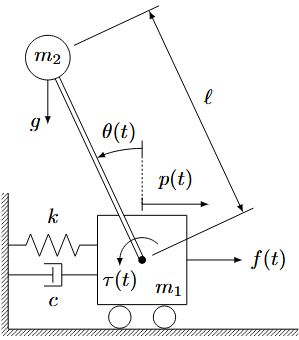
\includegraphics[width=0.5\linewidth]{msd_inv_pendulum.png}
    \caption{Inverted Pendulum on Cart System}
    \label{fig:msd_inv_pendulum}
\end{figure}
With two bodies (masses) in the system, we can describe the degrees of freedom and the velocities of each as:
\begin{align*}
    q_1(t) := p(t),& \quad \dot{q_1}(t) = \dot{p}(t), \\
    q_2(t) := \theta(t),& \quad \dot{q_2}(t) = \dot{\theta}(t), \\
    Q_1(t) := f(t),& \quad Q_2(t) := \tau(t), \\
    v_1 = \begin{bmatrix}
        \dot{p} \\ 0
    \end{bmatrix},& \quad
    v_2 = \begin{bmatrix}
        \dot{p} - \ell \dot{\theta}\cos(\theta) \\
        - \ell \dot{\theta}\sin(\theta)
    \end{bmatrix}
\end{align*}
Now, the components of the Euler-Lagrange equation (Eq. \ref{eq:eulerLagrangeFull}) can be found to assemble the complete equations of motion of the system.
\begin{equation*} 
    T_i = \frac{1}{2} m_{i} v^{T}_{i} v_{i} 
\end{equation*}
\begin{equation*}
    T_1 = \frac{1}{2}m_1 (\dot{p}^2 + 0^2), \quad T_2 = \frac{1}{2}m_2 [(\dot{p} - \ell\dot{\theta}\cos(\theta))^2 + (-\ell\dot{\theta}\sin(\theta))^2] 
\end{equation*}
The sum of the kinetic energy of the system is the sum of the kinetic energy of both masses:
\begin{align*}
    T &= T_1 + T_2 \\
    &= \frac{1}{2}m_1 \dot{p}^2 + \frac{1}{2}m_2[\dot{p}^2 - 2\ell \cos(\theta)\dot{p}\dot{\theta} + \ell^2\theta^2]
\end{align*}
We can then differentiate the above equation with respect to the generalized velocities $\dot{q_i}$. This gives us the following partial derivatives:
\begin{equation*}
    \frac{\partial T}{\partial\dot{q}_1} = (m_1 + m_2)\dot{p} - m_2\ell\dot{\theta}cos(\theta) \quad\textrm{and}\quad
    \frac{\partial T}{\partial\dot{q}_2} = m_2\ell[\ell\dot{\theta}-\cos(\theta)\dot{p}]
\end{equation*}
Differentiating again, with respect to time:
\begin{equation*} 
    \frac{d}{dt}(\frac{\partial T}{\partial\dot{q}_1}) = (m_1 + m_2)\ddot{p}-(m_2\ell)(\ddot{\theta}\cos(\theta)+\sin(\theta)\dot{\theta}^2) \quad\textrm{and}\quad \frac{d}{dt}(\frac{\partial T}{\partial\dot{q}_2}) = m_2\ell(\ell\ddot{\theta} - \ddot{p}\cos(\theta)-\dot{p}\sin(\theta))
\end{equation*}
Then, we also differentiate the total kinetic enery equation with respect to position:
\begin{equation*}
    \frac{\partial T}{\partial q_1} = 0 \quad\textrm{and}\quad \frac{\partial T}{\partial q_2} = m_2\ell\sin(\theta)\dot{\theta}\dot{p}
\end{equation*}
There are two sinks/sources of potential in the system. One is the spring, and the other is the gravitational potential of $m_2$. Thus, the total potential energy of the system is:
\begin{equation*}
V = \frac{1}{2}kq_1 + m_2 g \ell \cos(q_2)
\end{equation*}
This equation is differentiated with respect to position:
\begin{equation*}
    \frac{\partial V}{\partial q_1} = kp \quad\textrm{and}\quad \frac{\partial V}{\partial q_2} = -m_2 g\ell\sin(\theta)
\end{equation*}
There is one source of energy dissipation in the system: the damper. The energy dissipated by this component is given by:
\begin{equation*}
    R = \frac{1}{2}c\dot{p}^2
\end{equation*}
Differentiating this with respect to velocity:
\begin{equation*}
    \frac{\partial R}{\partial\dot{q}_1} = c \dot{p} \quad\textrm{and}\quad \frac{\partial R}{\partial\dot{q}_2} = 0
\end{equation*}
Now that all of the derivatives have been solved for, the nonlinear ODEs can be plugged into the Euler-Lagrange Equation, resulting in the coupled equations:
\begin{align*} 
    f &= (m_1 + m_2)\ddot{p} - m_2\ell \cos(\theta)\ddot{\theta} + m_2\ell \sin(\theta)\dot{\theta}^2 + c\dot{p} + kp \\
    \tau &= m_2\ell^2\ddot{\theta} - m_2\ell \cos(\theta)\ddot{p}-m_2 g\ell \sin(\theta)
\end{align*}
The coupled differential equations can be rearranged to isolate $\ddot{p}$ and $\ddot{\theta}$. In order to do this, the constants $\alpha(\theta)$ and $\beta(\theta)$ are defined as follows:
\begin{equation*}
    \alpha(\theta) := \frac{\cos(\theta)}{\ell} \quad\textrm{and}\quad \beta(\theta) := \frac{m_2 \ell \cos(\theta)}{m_1 + m_2}
\end{equation*}

These constants are used to eliminate the second derivative term in the coupled differential equations. Through some algebraic manipulation, it can be shown that the equations with the isolated second derivative are given by:

\begin{equation*} 
    \ddot{p} = \frac{m_2\ell\sin(\theta)[\alpha(\theta)g-\dot{\theta}^2]-c\dot{p}-kp+f+\alpha(\theta)\tau}{m_1 + m_2[1-\alpha(\theta)\ell\cos(\theta)]}
\end{equation*}

\begin{equation*} 
    \ddot{\theta} = \frac{m_2\ell \sin(\theta)[g - \beta (\theta)\dot{\theta}^2] + \beta (\theta)[f - c\dot{p}-kp] + \tau}{m_2\ell [\ell - \beta (\theta) \cos(\theta)]}
\end{equation*}
These are the final equations of motion, without solving for the reaction force of the pendulum on the cart!

\end{document}